\chapter{Results and physics interpretations}
In this chapter, we present our results after all corrections discussed above and including
all systematic errors. In order to discuss these results, we first present the functional forms
we will use to fit them, which are different for the coherent and incoherent 
channels. For the coherent channel, we use exact formula from \cite{FX_BSA} to 
extract the real and imaginary parts
of the CFF $\mathcal{H}_{A}$ at twist-2. For the incoherent channel, we use a simplified form 
and only extract the asymmetry at $90^{\circ}$. Then we present the beam-spin asymmetry 
measurements for both DVCS channels with their aforementioned fits and draw some first 
conclusions. Finally we present ratios of our asymmetry to free proton results 
from CLAS (E1-DVCS part-1 \cite{FX_BSA, FX_analysis_note}).

\section{Fitting the beam-spin asymmetry} \label{Beam-Spin}
For a spin-zero target at leading twist, the beam-spin asymmetry ($A_{LU}$) 
can be expressed as follow \cite{BM_2009}
\begin{equation}
A_{LU}(\phi) = \frac{\alpha_{0}(\phi) \, \Im m(\mathcal{H}_{A})}
{\alpha_{1}(\phi) + \alpha_{2}(\phi) \, \Re e(\mathcal{H}_{A}) + \alpha_{3}(\phi) \, 
\big( 
\Re e(\mathcal{H}_{A})^{2} + \Im m(\mathcal{H}_{A})^{2} \big)}
\label{eq:A_LU-coh}
\end{equation}
where $\Im m(\mathcal{H}_{A})$ and $\Re e(\mathcal{H}_{A})$ are the imaginary 
and real parts of the CFF $\mathcal{H}_{A}$ associated to the GPD $H_A$. The 
$\alpha_{i}$'s are $\phi$-dependent kinematical factors that depend on the 
nuclear form factor $F_A$ and the independent variables $Q^2$, $x_{B}$ and $t$.  
These factors are simplified as:

\small
\begin{eqnarray}
   \alpha_0 (\phi) & = &\frac{x_{A}(1+\epsilon^2)^2}{y} S{++}(1) \sin(\phi)\\
    \alpha_1 (\phi) & = & c_0^{BH}+c_1^{BH} \cos({\phi})+c_2^{BH} \cos(2\phi)\\ 
   \alpha_2 (\phi) & = & \frac{x_{A}(1+\epsilon^2)^2}{y}  \left( C_{++}(0) +  
C_{++}(1) cos(\phi) \right)\\
\alpha_3 (\phi) &=& \frac{x^{2}_{A}t(1+\epsilon^2)^2}{y} {\mathcal P}_1(\phi) 
{\mathcal P}_2(\phi) \cdot 2 \frac{2-2y+y^2 + \frac{\epsilon^2}{2}y^2}{1 + 
\epsilon^2}
\end{eqnarray}
\normalsize

Where $S{++}(1)$, $C_{++}(0)$, and $C_{++}(1)$ are the Fourier harmonics in the 
leptonic tensor. Their explicit expressions can be found in Appendix 
\ref{app:Helium_cross_section}.  

Using the $\alpha_{i}$ factors, one can obtain in a model-independent way $\Im
m(\mathcal{H}_{A})$ and $\Re e(\mathcal{H}_{A})$ from fitting the experimental 
$A_{LU}$ as a function of $\phi$ for given values of $Q^2$, $x_B$ and $t$.  
Equation \ref{eq:A_LU-coh} is the functional form we use to fit the coherent asymmetries 
presented in this analysis. 

Regarding the incoherent channel, the beam-spin 
asymmetry signals will be fitted by the simple form $\frac{\alpha \sin(\phi)}{1 + 
\beta \cos(\phi)}$, which has been used for DVCS on free proton, see reference 
\cite{FX_BSA, FX_analysis_note}, and allows an easy extraction of 
$A^{90^{\circ}}_{LU}$.  


\section{Beam-spin asymmetry results and fit}
In this section, the beam-spin asymmetries will be compared to the theoretical calculations based on the two models that were presented in section \ref{Theoretical_hypotheses}.

\subsection{Coherent beam-spin asymmetry}
Figure \ref{fig:bsa_coh_Q2_bins} shows the coherent $A_{LU}$ for the three 
sets of two-dimensional bins. The asymmetries are fitted with the form of
equation \ref{eq:A_LU-coh}, where the real and the imaginary part of the CFF 
$\mathcal{H}_{A}$ are the free parameters in the fit.

\begin{figure}[tpb]
\centering
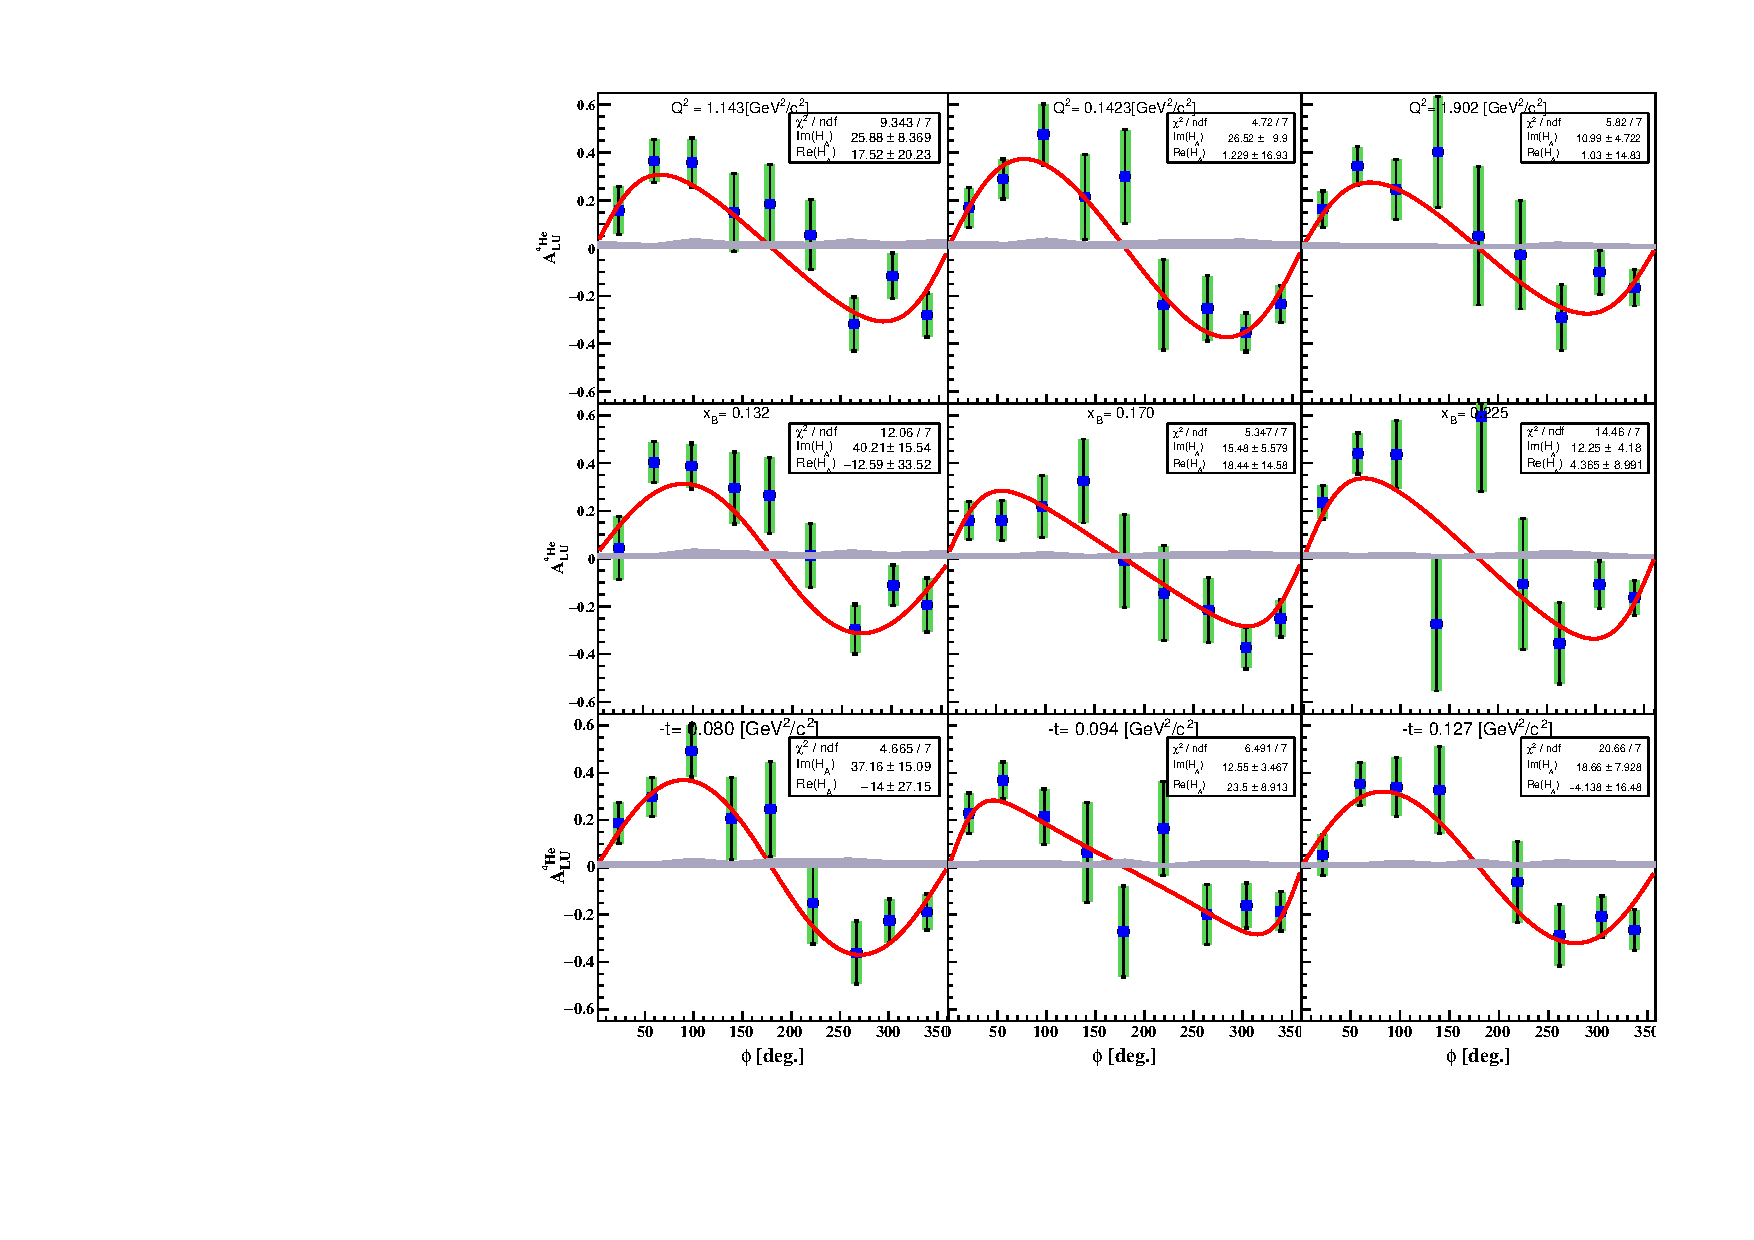
\includegraphics[scale=0.9]{fig_Dec2016/Coherent_ALU_phi.pdf}
\caption{The coherent $A_{LU}$ as a function of $\phi$ and $Q^2$ (top panel), 
   $x_{B}$ (middle panel), and $-t$~(bottom panel) bins. The blue error bars 
   represent the statistical and the systematic uncertainties, added 
   quadratically, shown on the top of green error bars representing only the 
statistical uncertainties.  The brown bands represent the full systematic 
uncertainties, including the normalisation systematic uncertainties. The red 
curves represent fits in the form of equation \ref{eq:A_LU-coh}.}
\label{fig:bsa_coh_Q2_bins}
\end{figure}

Figure \ref{fig:coh_Q2_xB_t_ALU} shows the $Q^2$, $x_{B}$, and 
$-t$-dependencies of the $\alpha$ term of $A_{LU}$. The $x_{B}$ and 
$-t$-dependencies are compared to theoretical calculations performed by S.  
Liuti and K. Taneja. Their model relies on the impulse approximation and uses 
advanced spectral function of the nuclei to calculate the nuclear GPDs and then 
the observables. The calculations were carried out at slightly different 
kinematics than ours but provide already some guidance. The experimental 
results appear to have larger asymmetries compared to the calculations. These 
differences may arise from nuclear effects which are not taken into account in 
the model, such as long-range interactions \cite{simonetta_2}. Our measurements 
also agree with those of HERMES, considering their large uncertainties. 

\begin{figure}[tpb]
\centering
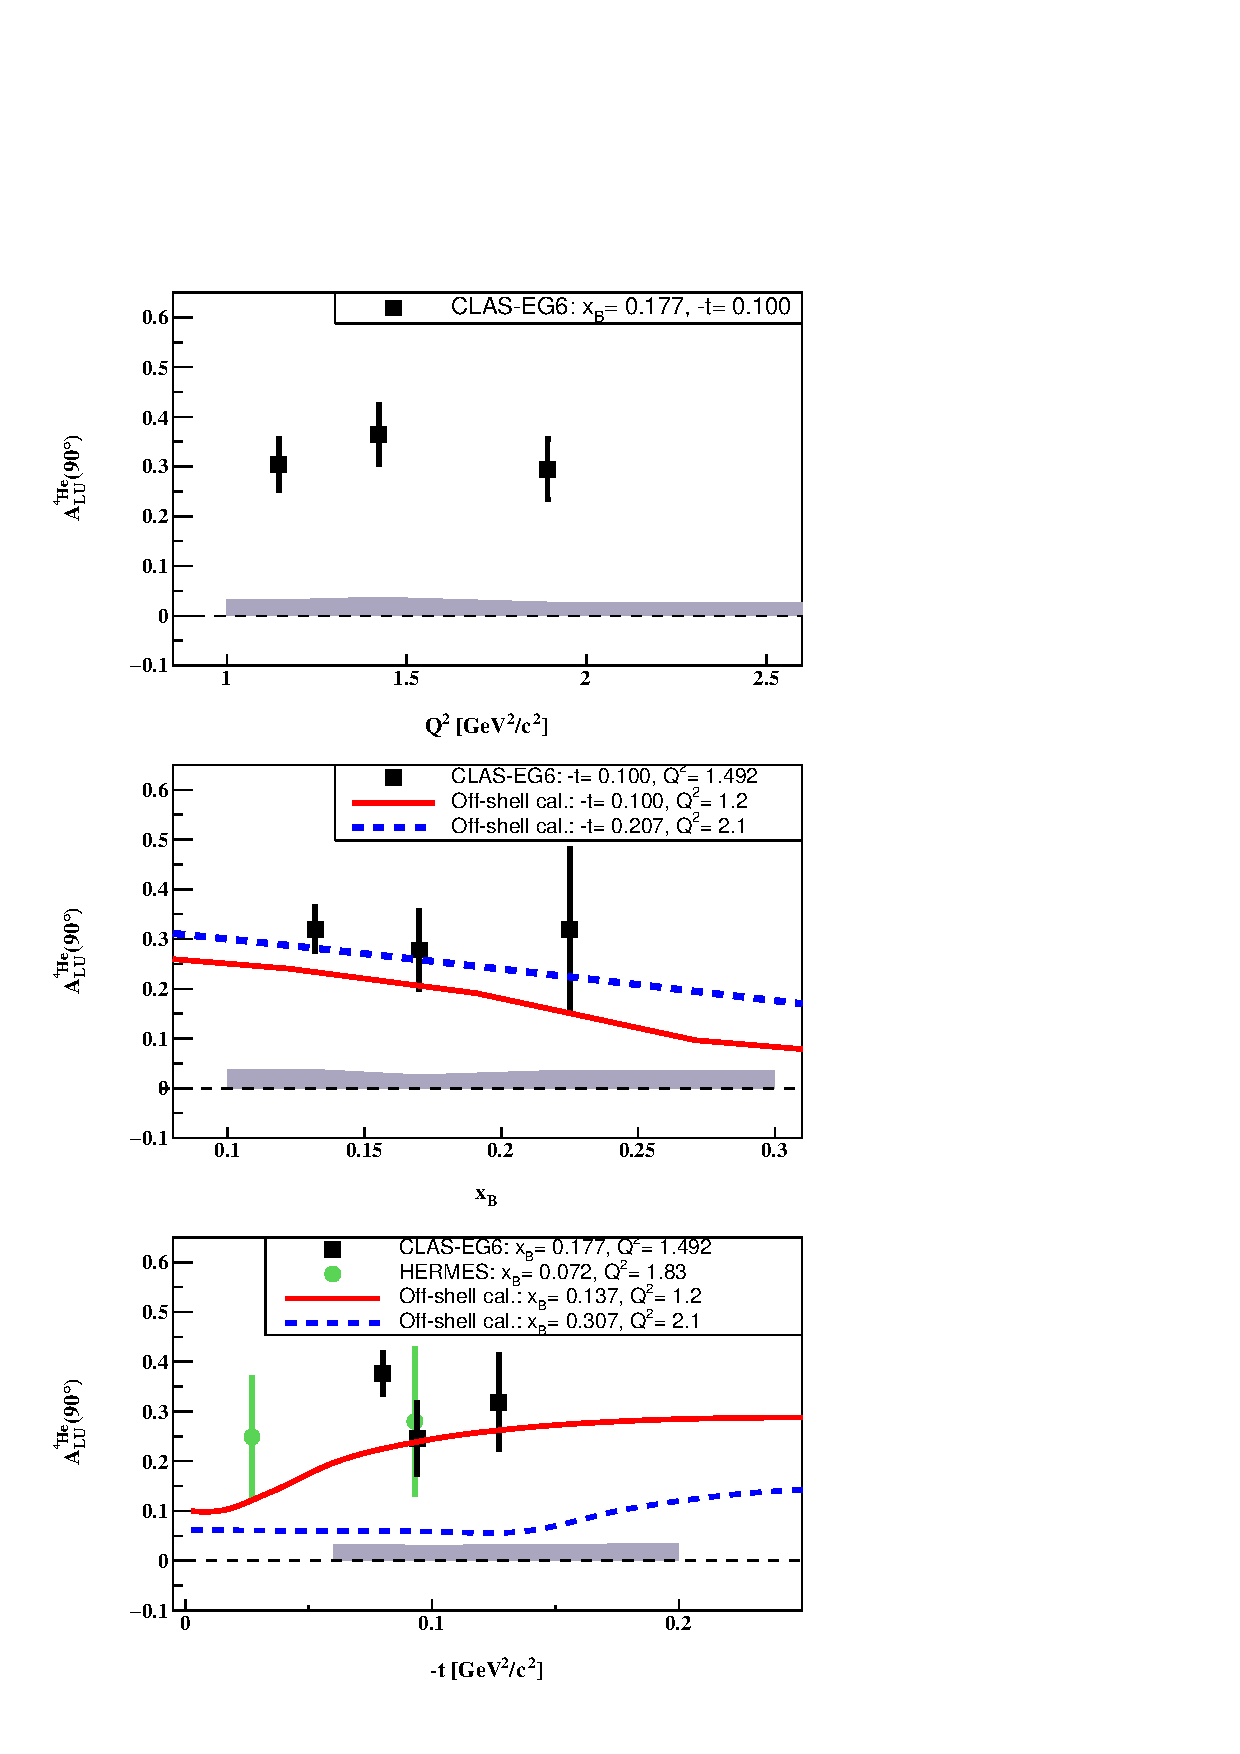
\includegraphics[scale=0.9]{fig_Dec2016/Coherent_ALU_phi_90.pdf}
   \caption{The $Q^{2}$-dependence (on the top), the $x_{B}$-dependence (on the 
      middle), and the $t$-dependence~(on the bottom) of the fitted coherent 
      $A_{LU}$ signals at $\phi$= 90$^{\circ}$ (black squares). On the middle: 
      the red and the blue curves are theoretical predictions from 
      \cite{simonetta_2} at two values of $-t$. On the bottom: the green 
      circles are the HERMES $-A_{LU}$ (positron beam was used) inclusive 
      measurements \cite{HERMES_BSA}, and the colored curves represent 
      theoretical predictions from \cite{simonetta_2}.} 
      \label{fig:coh_Q2_xB_t_ALU}
\end{figure}


\subsection{Incoherent beam-spin asymmetry}
Figure \ref{fig:bsa_incoh_bins} shows our measured incoherent beam-spin 
asymmetries, for the three sets of the two-dimensional bins as for the coherent 
channel. The $Q^2$, $x_{B}$, and $-t$-dependencies of $A_{LU}$ at 
$\phi$=~90$^{\circ}$ (the $\alpha$ parameter of the fit) are shown in figure 
\ref{fig:incoh_Q2_xB_t_ALU}.

The theoretical calculations from S. Liuti and K. Taneja are carried out at 
slightly different kinematics than our experimental measured values.  
Nevertheless, one can see that our incoherent asymmetries are not well 
described by these calculations. For instance, in the top right plot of figure 
\ref{fig:incoh_Q2_xB_t_ALU}, even though our asymmetries (at 
$-t$~=~0.2~GeV$^2$/c$^2$) are located between the model's predictions, which 
are carried out at $-t$~=~0.095 and 0.329~GeV$^2$/c$^2$, they do not show the 
drop in $<x_B>$, as the model predicted. Similar observation can be seen as a 
function of $-t$ from the bottom plot.

\begin{figure}[tpb]
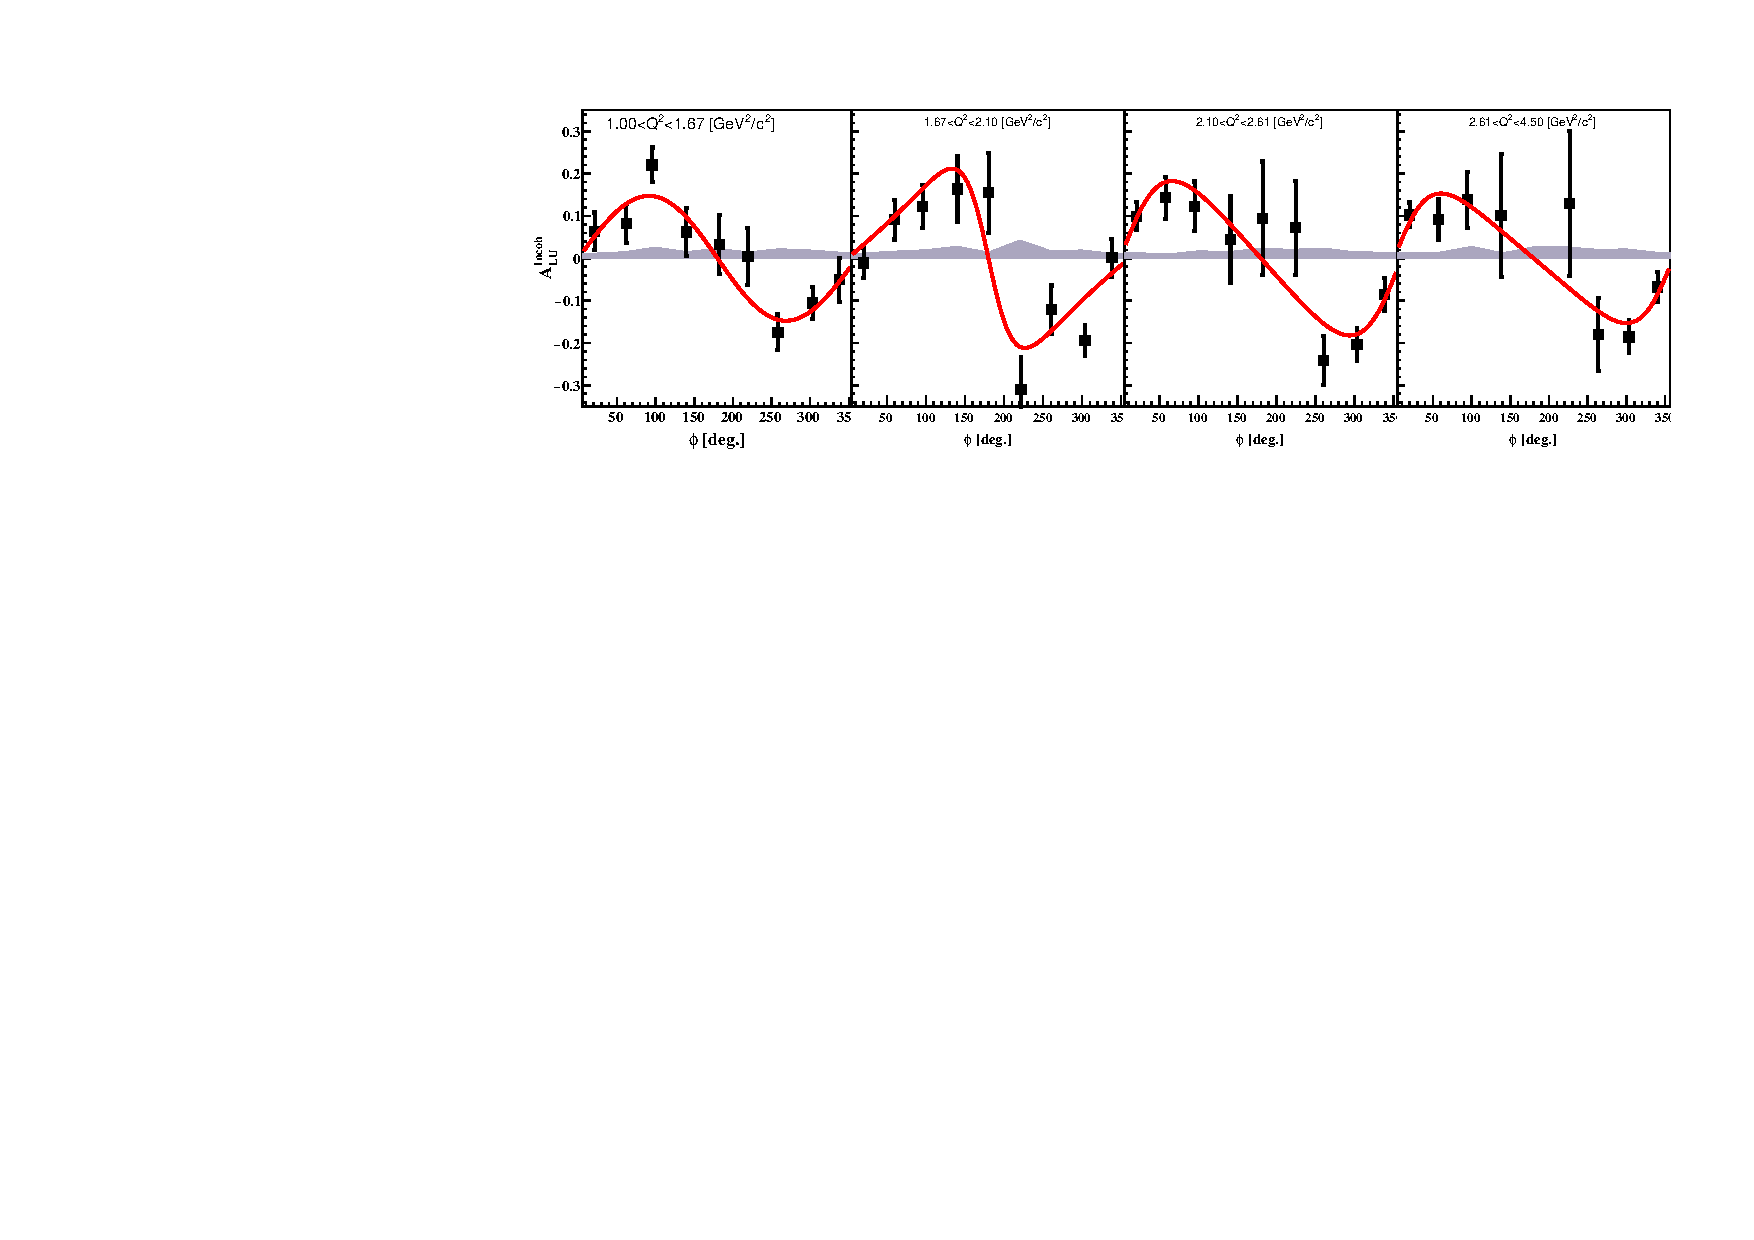
\includegraphics[scale=0.9]{fig_Dec2016/ALU_phi_p_Q2.pdf}
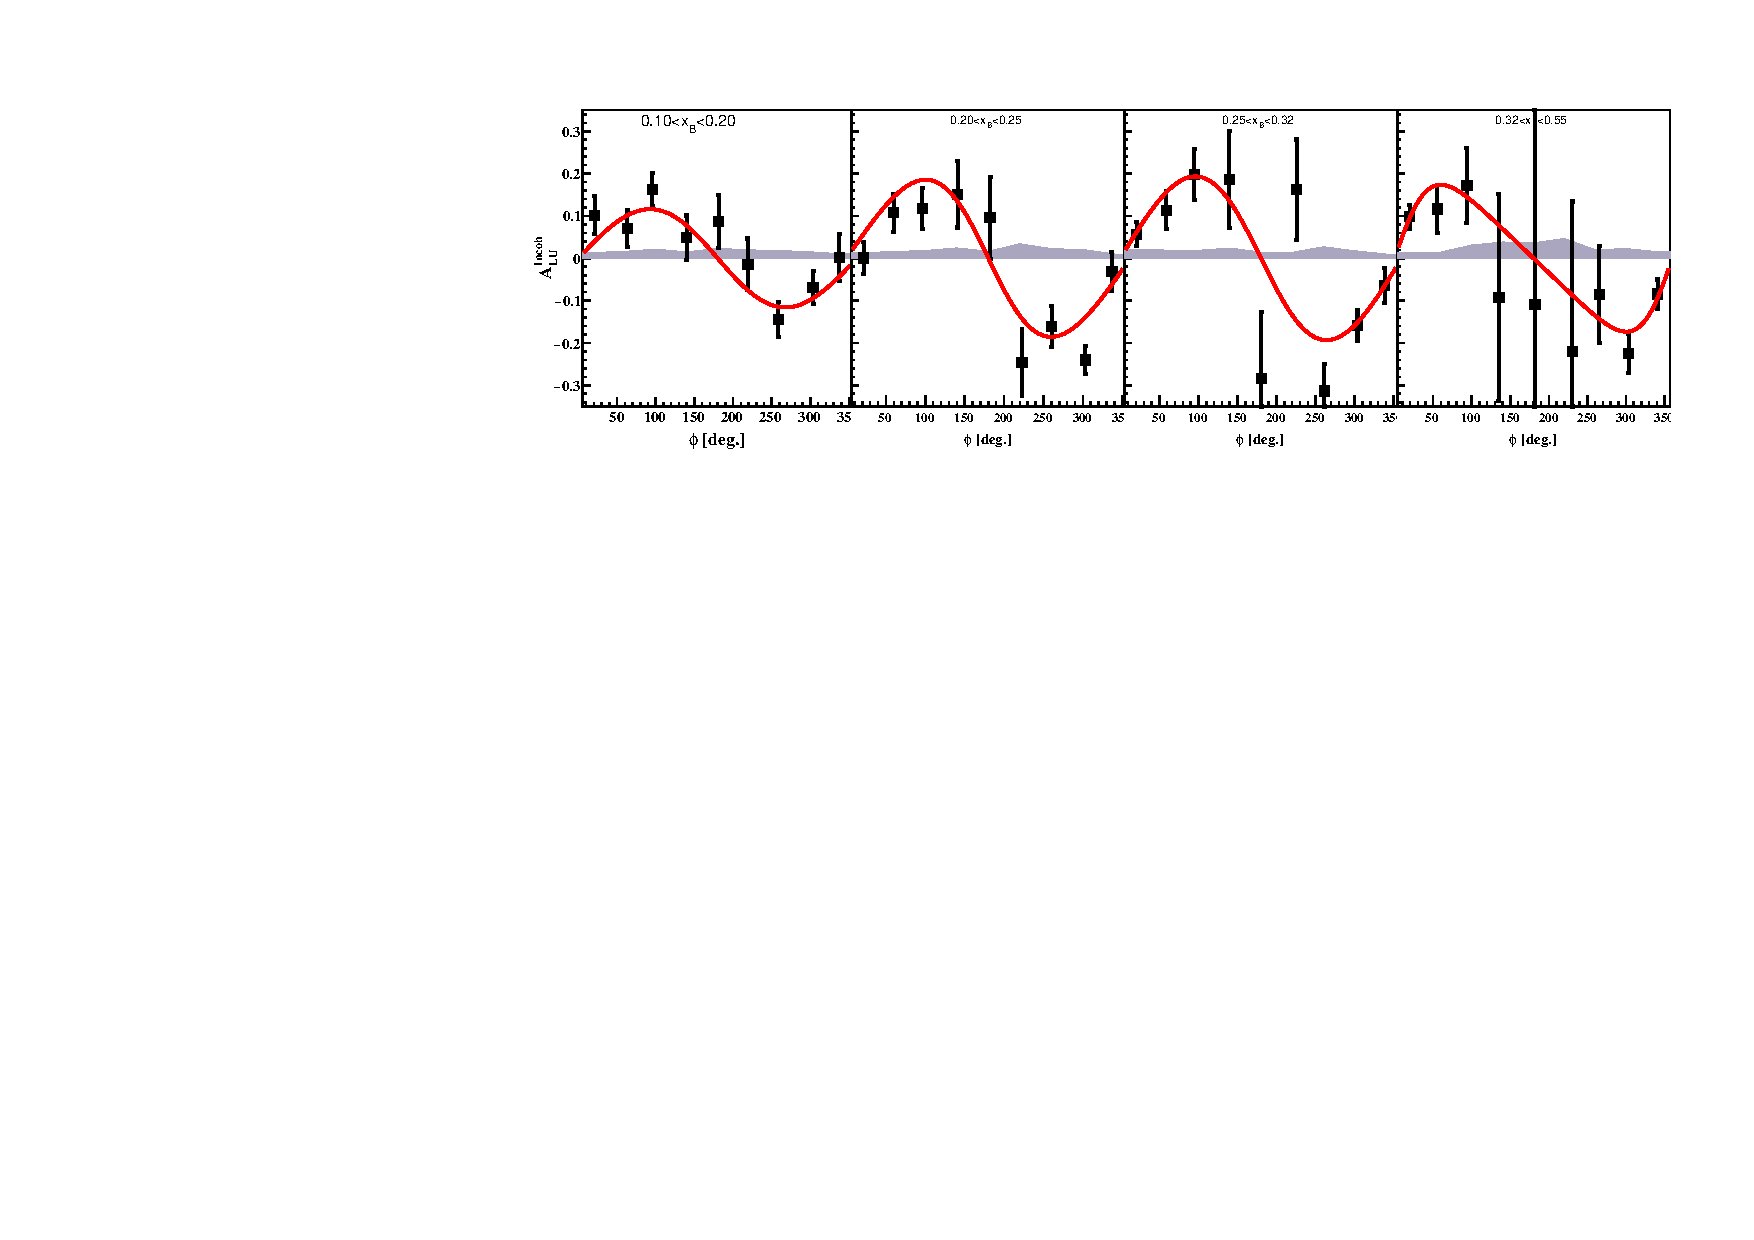
\includegraphics[scale=0.9]{fig_Dec2016/ALU_phi_p_x.pdf}
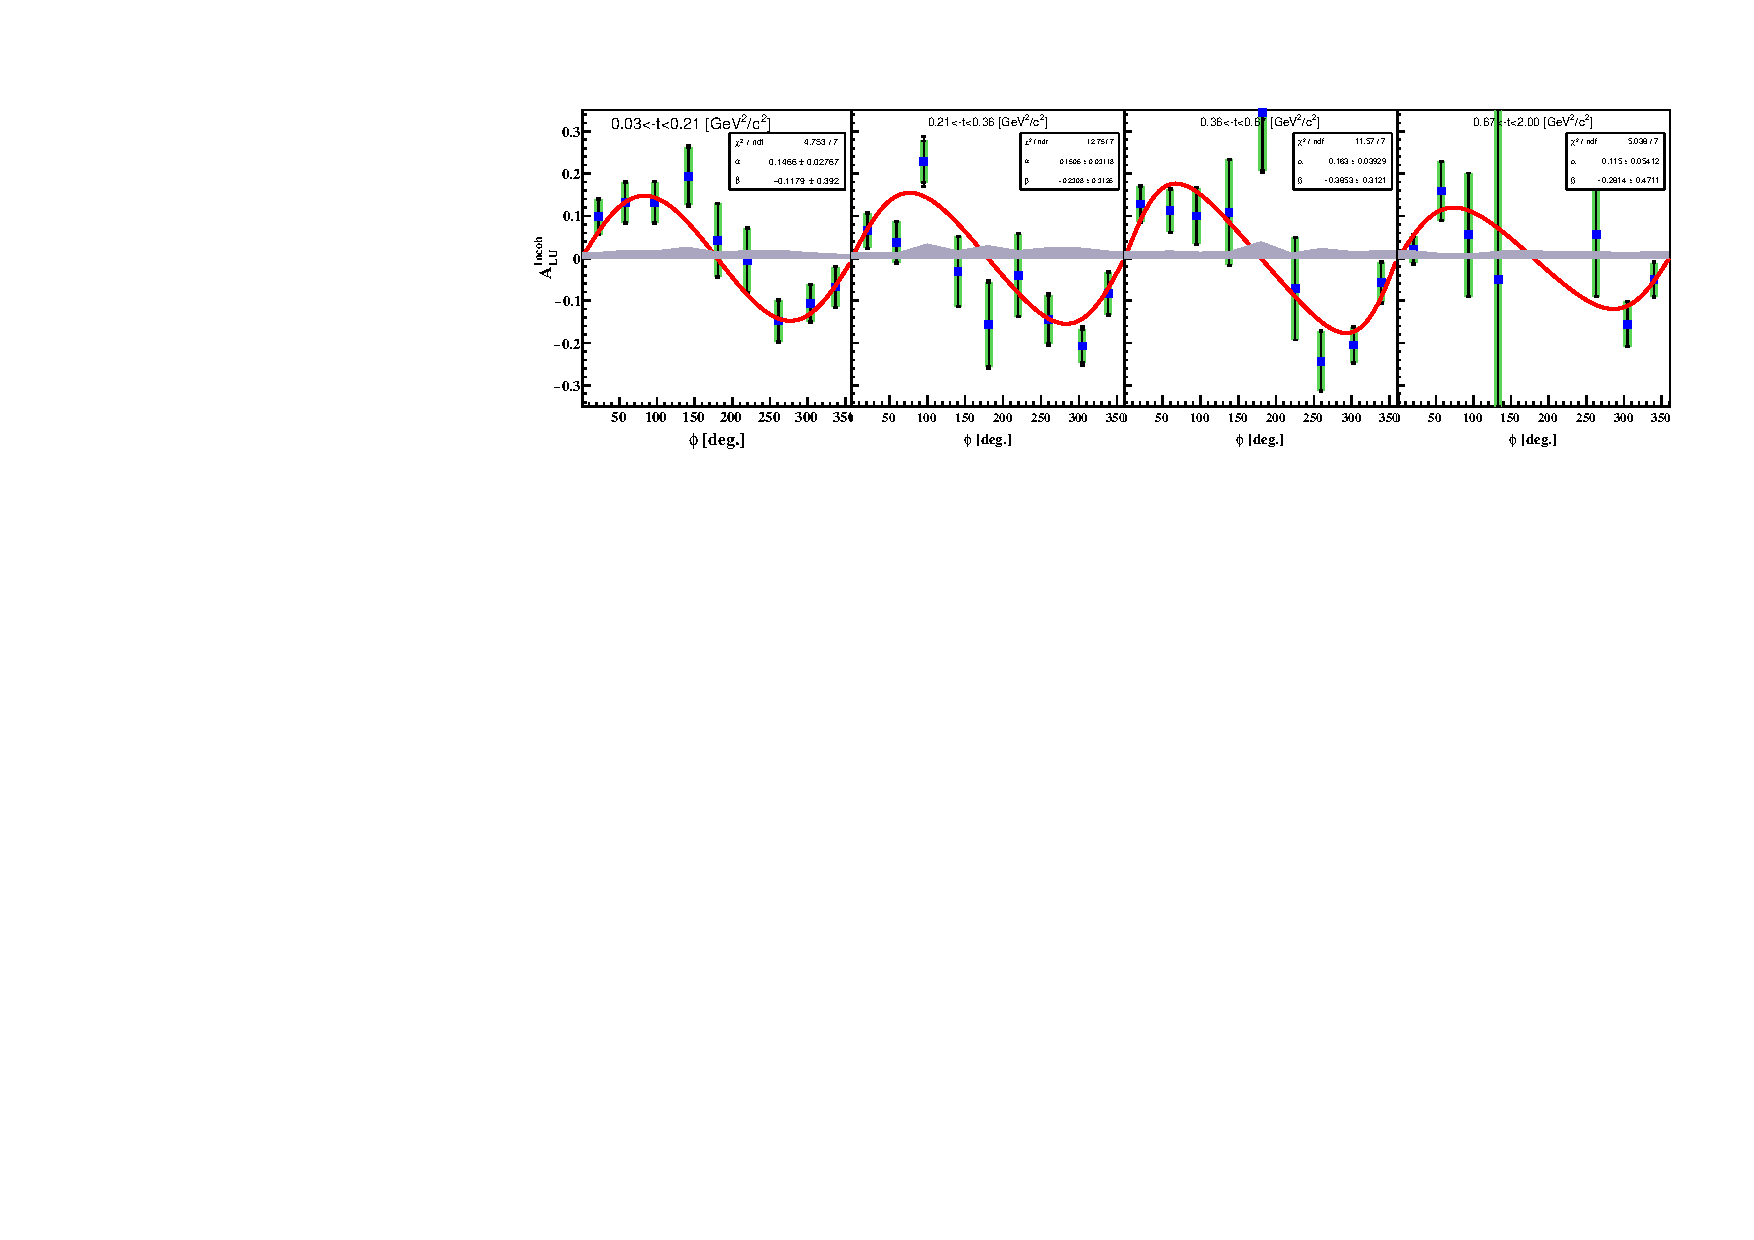
\includegraphics[scale=0.9]{fig_Dec2016/ALU_phi_p_t.pdf}
\caption{The incoherent $A_{LU}$ as a function of the angle $\phi$ in $Q^2$, 
   $x_B$, and $-t$ bins, respectively from top to bottom. See the caption of 
   figure \ref{fig:bsa_coh_Q2_bins} for the color indications. The red lines 
   represent fits to the $\frac{\alpha \sin(\phi)}{1 + \beta cos(\phi)}$ 
   function.  } \label{fig:bsa_incoh_bins}
\end{figure}

\begin{figure}[tpb]
   \centering
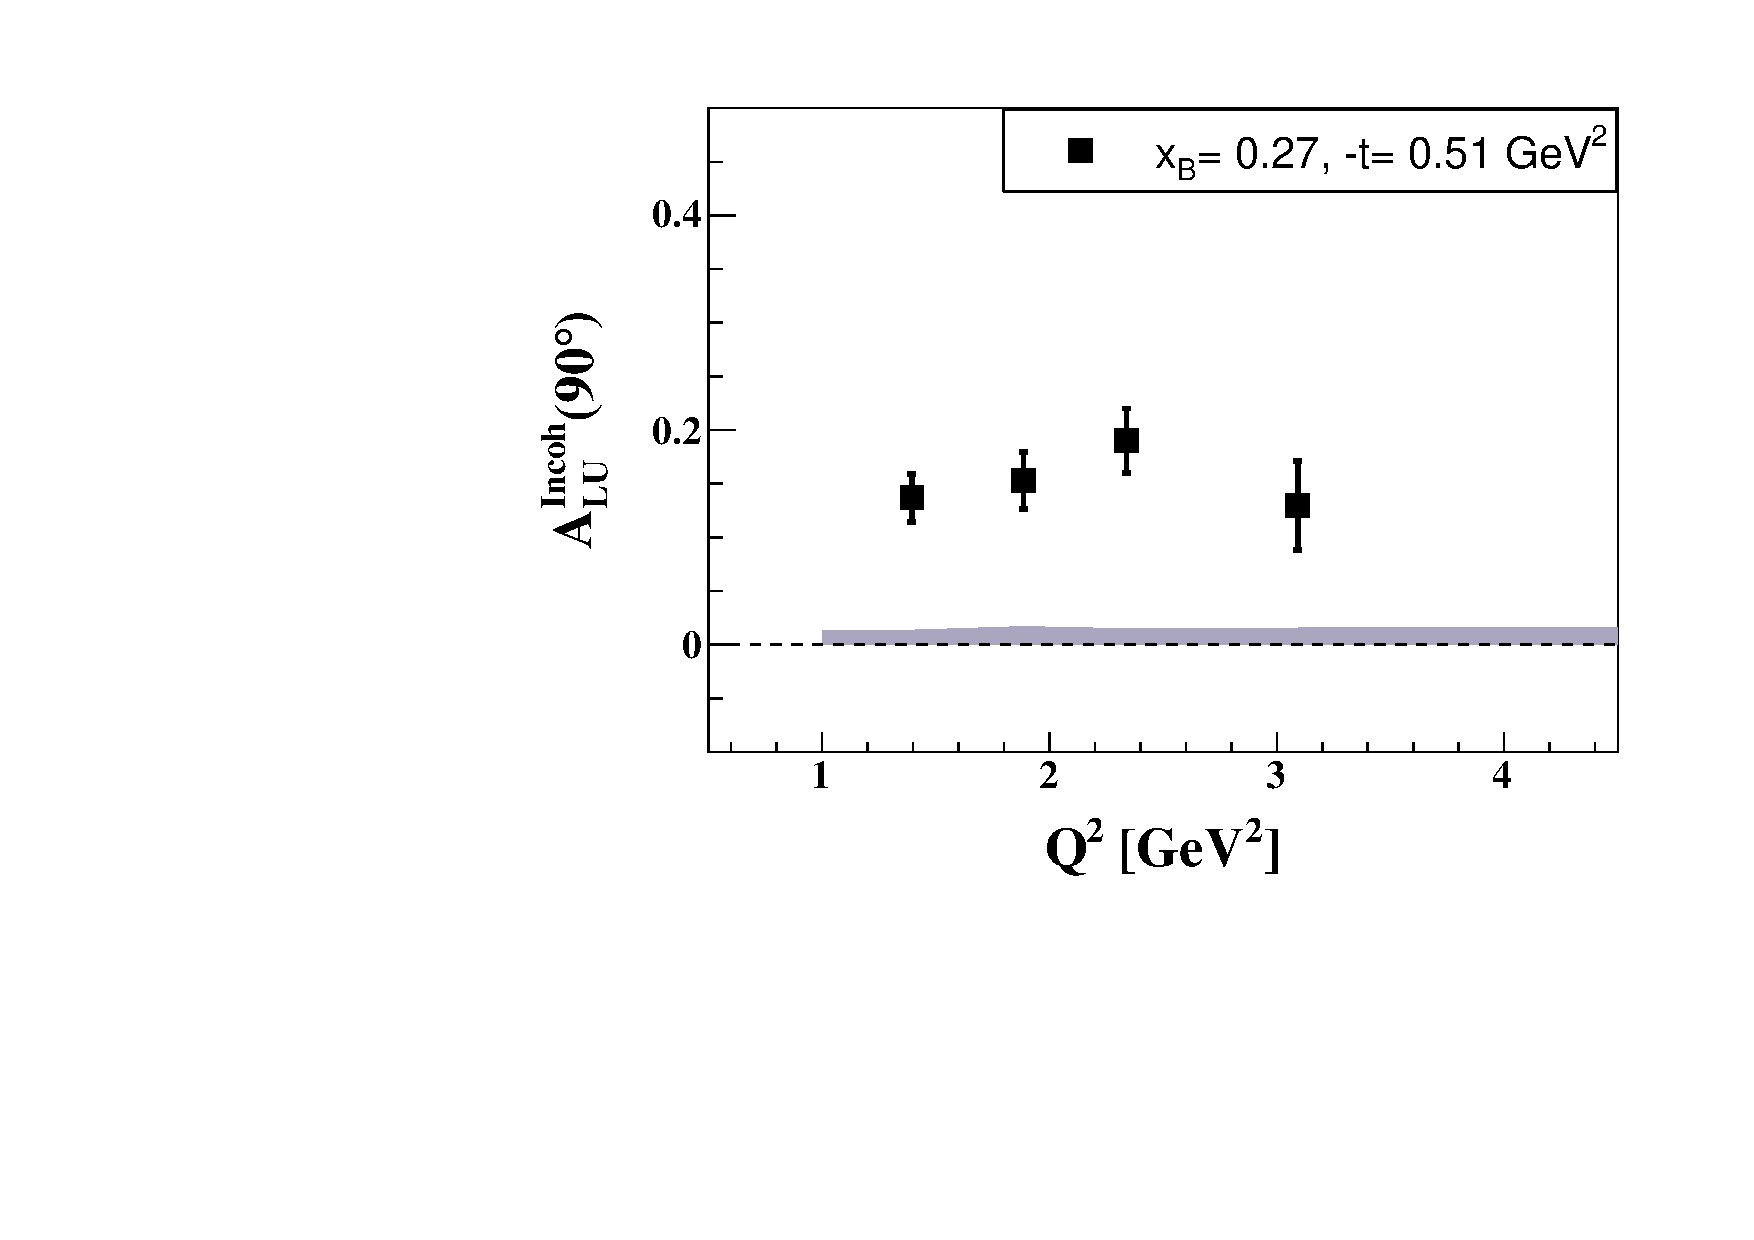
\includegraphics[scale=0.48]{fig_Dec2016/ALU_90_p_vs_Q2_shortscenrario.pdf}\\ 
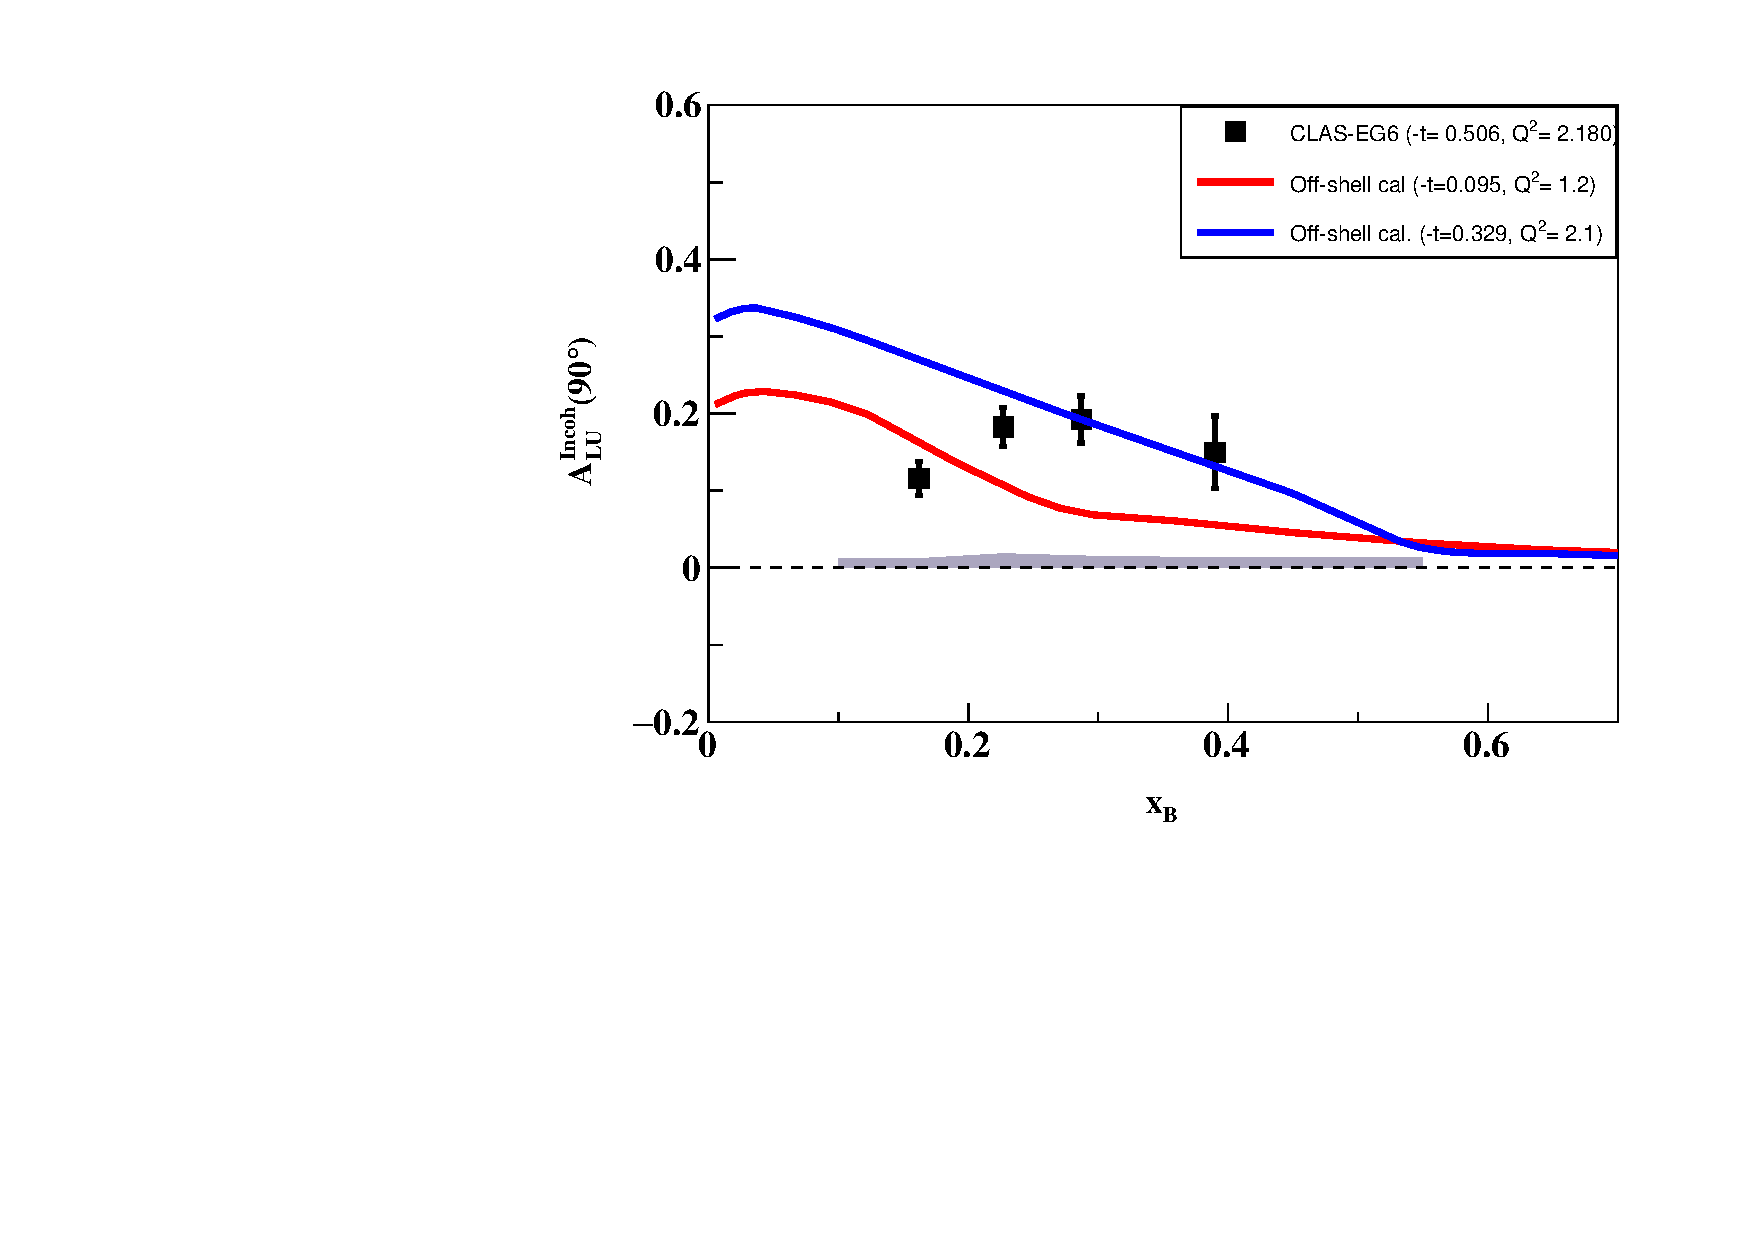
\includegraphics[scale=0.48]{fig_Dec2016/ALU_90_p_vs_x_shortscenrario.pdf}\\
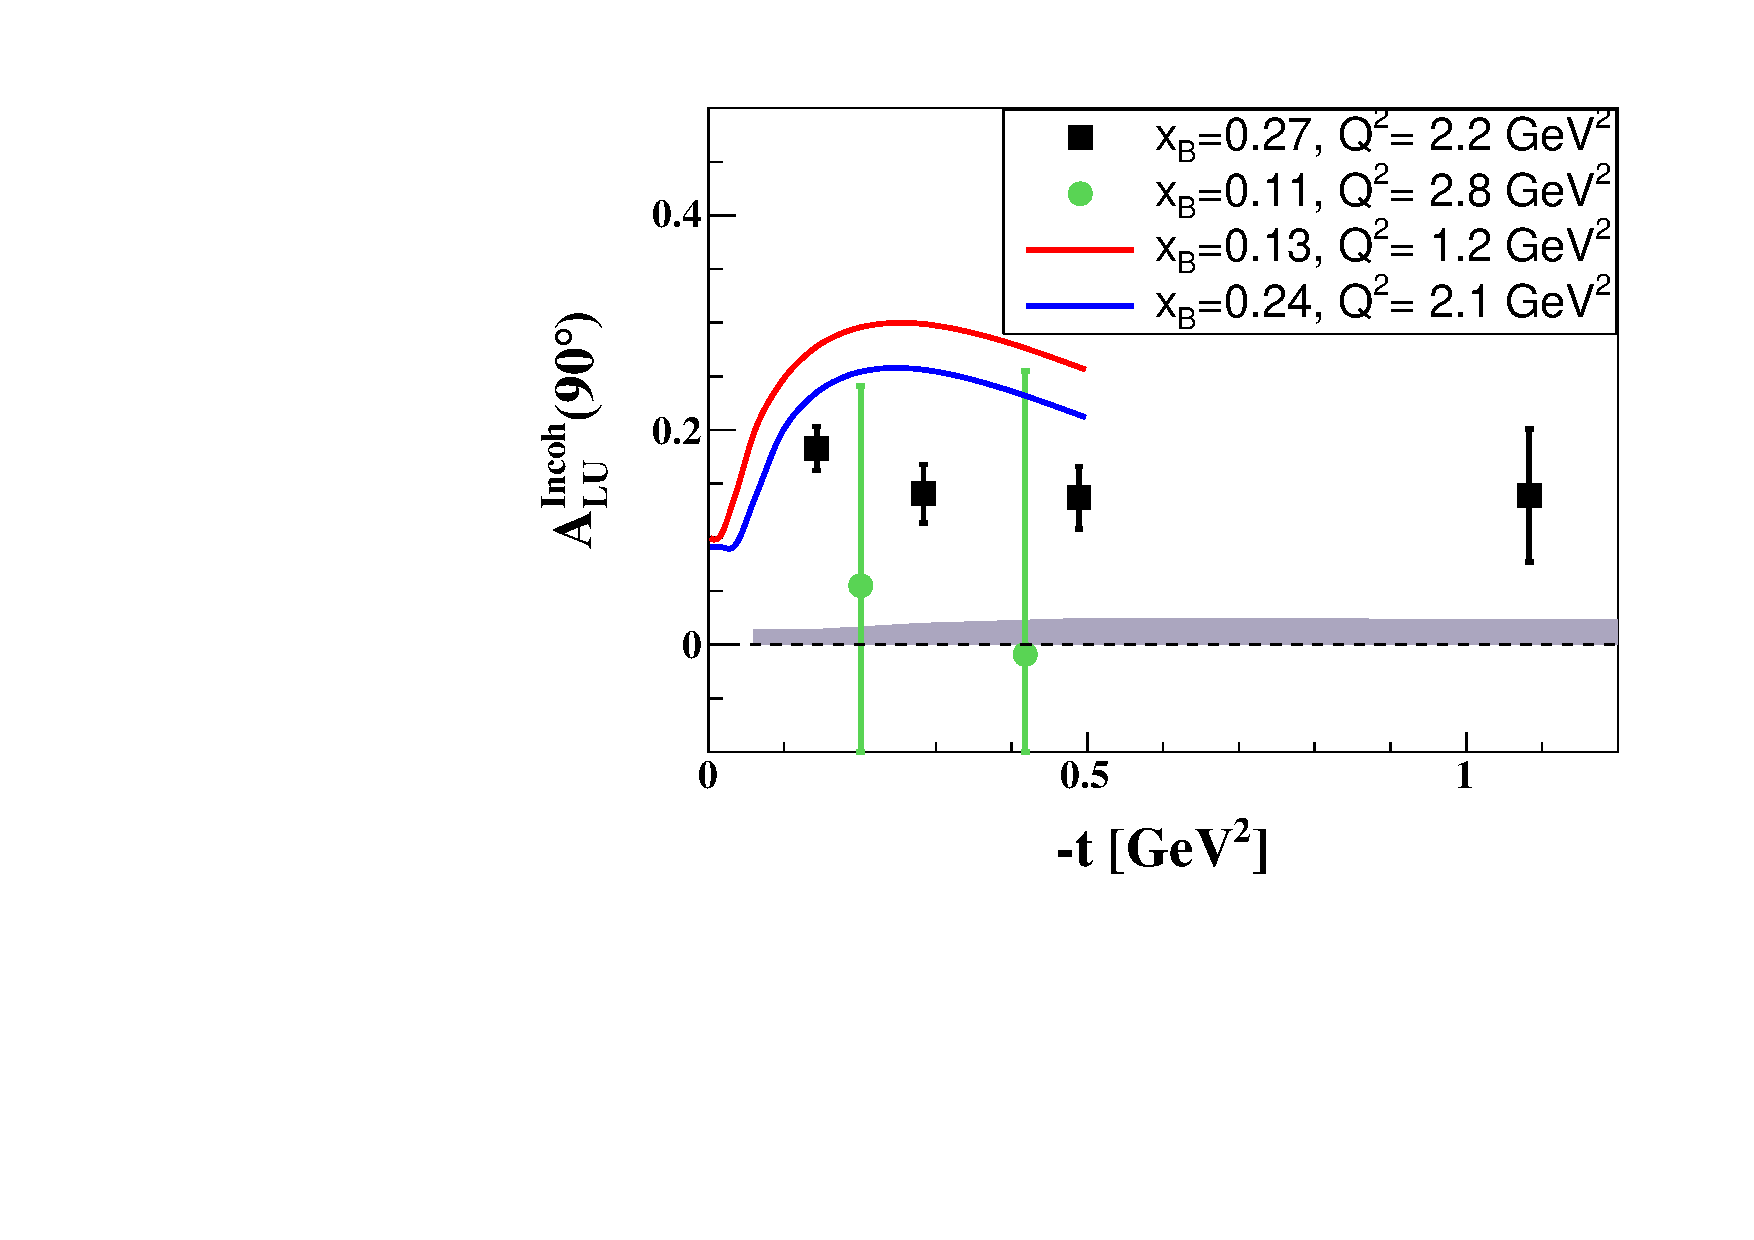
\includegraphics[scale=0.48]{fig_Dec2016/ALU_90_p_vs_t_shortscenrario.pdf} \\ 
\caption{The $Q^{2}$ (top), $x_{B}$ (middle), and $-t$-dependencies (bottom) of 
   the incoherent $A_{LU}$ at $\phi$~=~90$^{\circ}$ (black squares). Middle 
   panel: the red and the blue curves are theoretical calculations from 
   \cite{simonetta_2}. On the bottom: the green circles are the HERMES 
   $-A_{LU}$ (positron beam was used) inclusive measurements \cite{HERMES_BSA}, 
   the colored curves represent theoretical calculations from 
\cite{simonetta_2}.  } \label{fig:incoh_Q2_xB_t_ALU}
\end{figure}


\section{Helium GPD}
As shown at the beginning of this chapter, one can extract both real and
imaginary parts of the $^4$He CFF $\mathcal{H}_A$ from fitting the beam-spin 
asymmetry signals. This extraction is fully model independent and, in contrast 
with the proton's GPD extraction, does not make any assumption on additional 
GPDs. In this work, we performed the first experimental extraction of 
$\mathcal{H}_A$ from exclusive measurements of the reaction. The results are 
presented in figure \ref{fig:HA_CFF} as function of $Q^{2}$, $x_B$, and $-t$.

Within the given uncertainties, our results show a slight dependence on 
$Q^{2}$, $x_B$, and $-t$, which are in agreement with the theoretical 
calculations for $\mathcal{H}_A$.  One can see a difference between the 
precision of the extracted real and imaginary parts, indicating the fact that 
the beam-spin asymmetry is mostly sensitive to the imaginary part of the CFF 
$\mathcal{H}_A$.

\begin{figure}[h!]
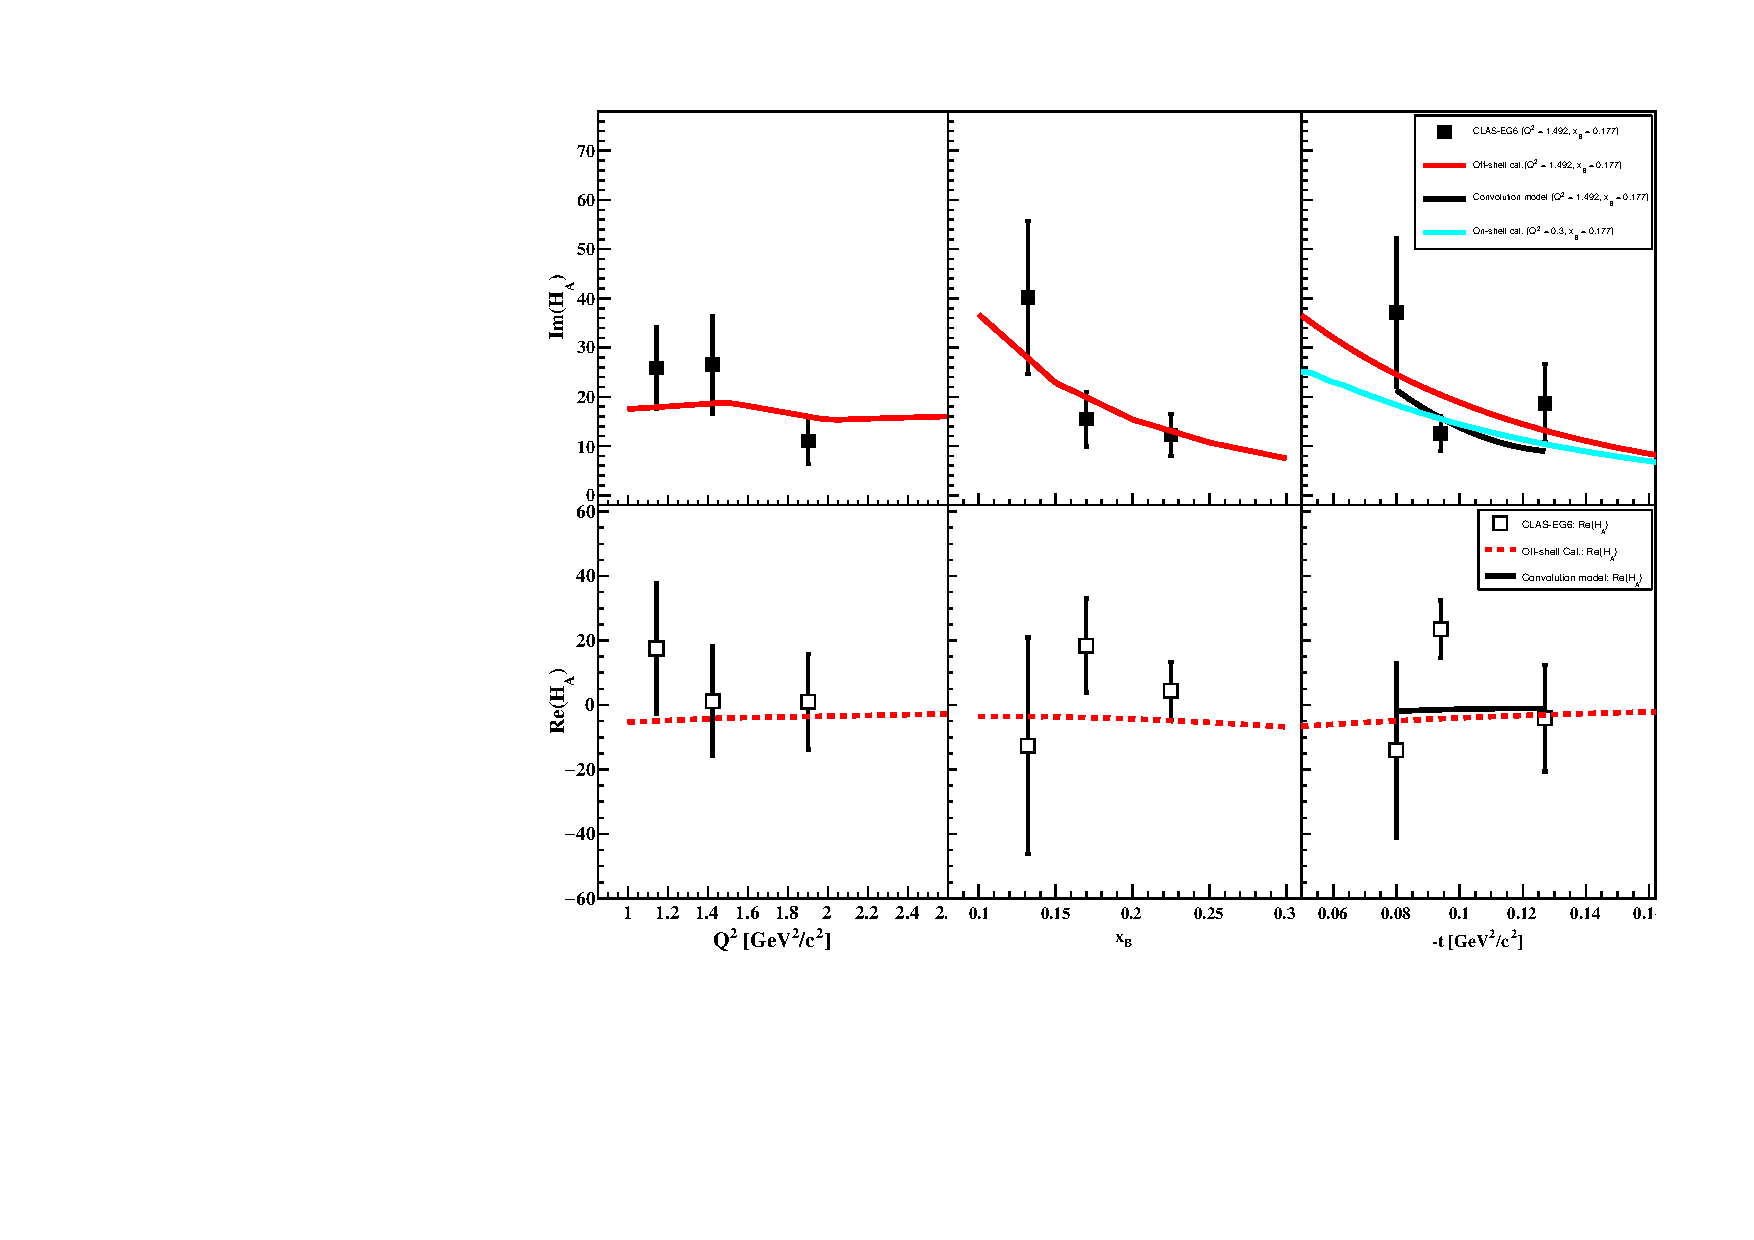
\includegraphics[scale=0.9]{fig_Dec2016/Coherent_CFF.pdf}
\caption{The model-independent extraction of the imaginary (black full squares 
in the top panel plots) and real (empty black squares in the bottom panel 
plots) parts of the $^4$He CFF $\mathcal{H}_A$, as functions of $Q^{2}$ (on the 
left), $x_B$ (on the middle), and $t$ (on the right). The full and dashed red 
curves are calculations based on the impulse approximation from 
\cite{Vadim_priv}.  The black curves in the right plots, t-dependence plots, 
are calculations from a convolution model based on the VGG model for the 
nucleon's GPDs \cite{Guidal_priv}. The cyan curve on the top-right plot is from 
the off-shell calculations presented in section \ref{Theoretical_hypotheses} 
based on reference \cite{GonzalezHernandez:2012jv}.  }
\label{fig:HA_CFF}
\end{figure}


\section{Generalized EMC ratios} \label{sec:Generalized_EMC}
Comparing our measured DVCS channels to the free-proton DVCS reaction 
allows us to investigate the nuclear medium effects at the GPD level. For this 
we use analyzes performed on free-proton with the DVCS data sets taken by the CLAS 
collaboration, during the E1-DVCS experiment (parts 1 and 2). The results of 
part 1 are already published \cite{FX_BSA, CLAS_cross_section}. Herein, our 
coherent and incoherent beam-spin asymmetries are compared to the results of
free proton asymmetries from this publication.


The explored kinematical ranges of $Q^2$, $x_{B}$ and $-t$ of the free-proton 
data are similar to the ones of the incoherent channel, and the two data sets 
were recorded using similar electron-beam energies and experimental setup.  
Therefore, we construct $A_{LU}$ ratios based on choosing the free proton bins 
which have similar $Q^2$, $x_{B}$ and $-t$ values as our bins. The incoherent 
$A_{LU}$ ratios at $\phi$~=~90$^{\circ}$ are shown in figure 
\ref{fig:incoh_EMC_ratio_ALU_proton} as functions of $Q^{2}$, $x_{B}$, and 
$-t$, along with theoretical predictions at similar kinematical values.
  
\begin{figure}[tp]
\centering
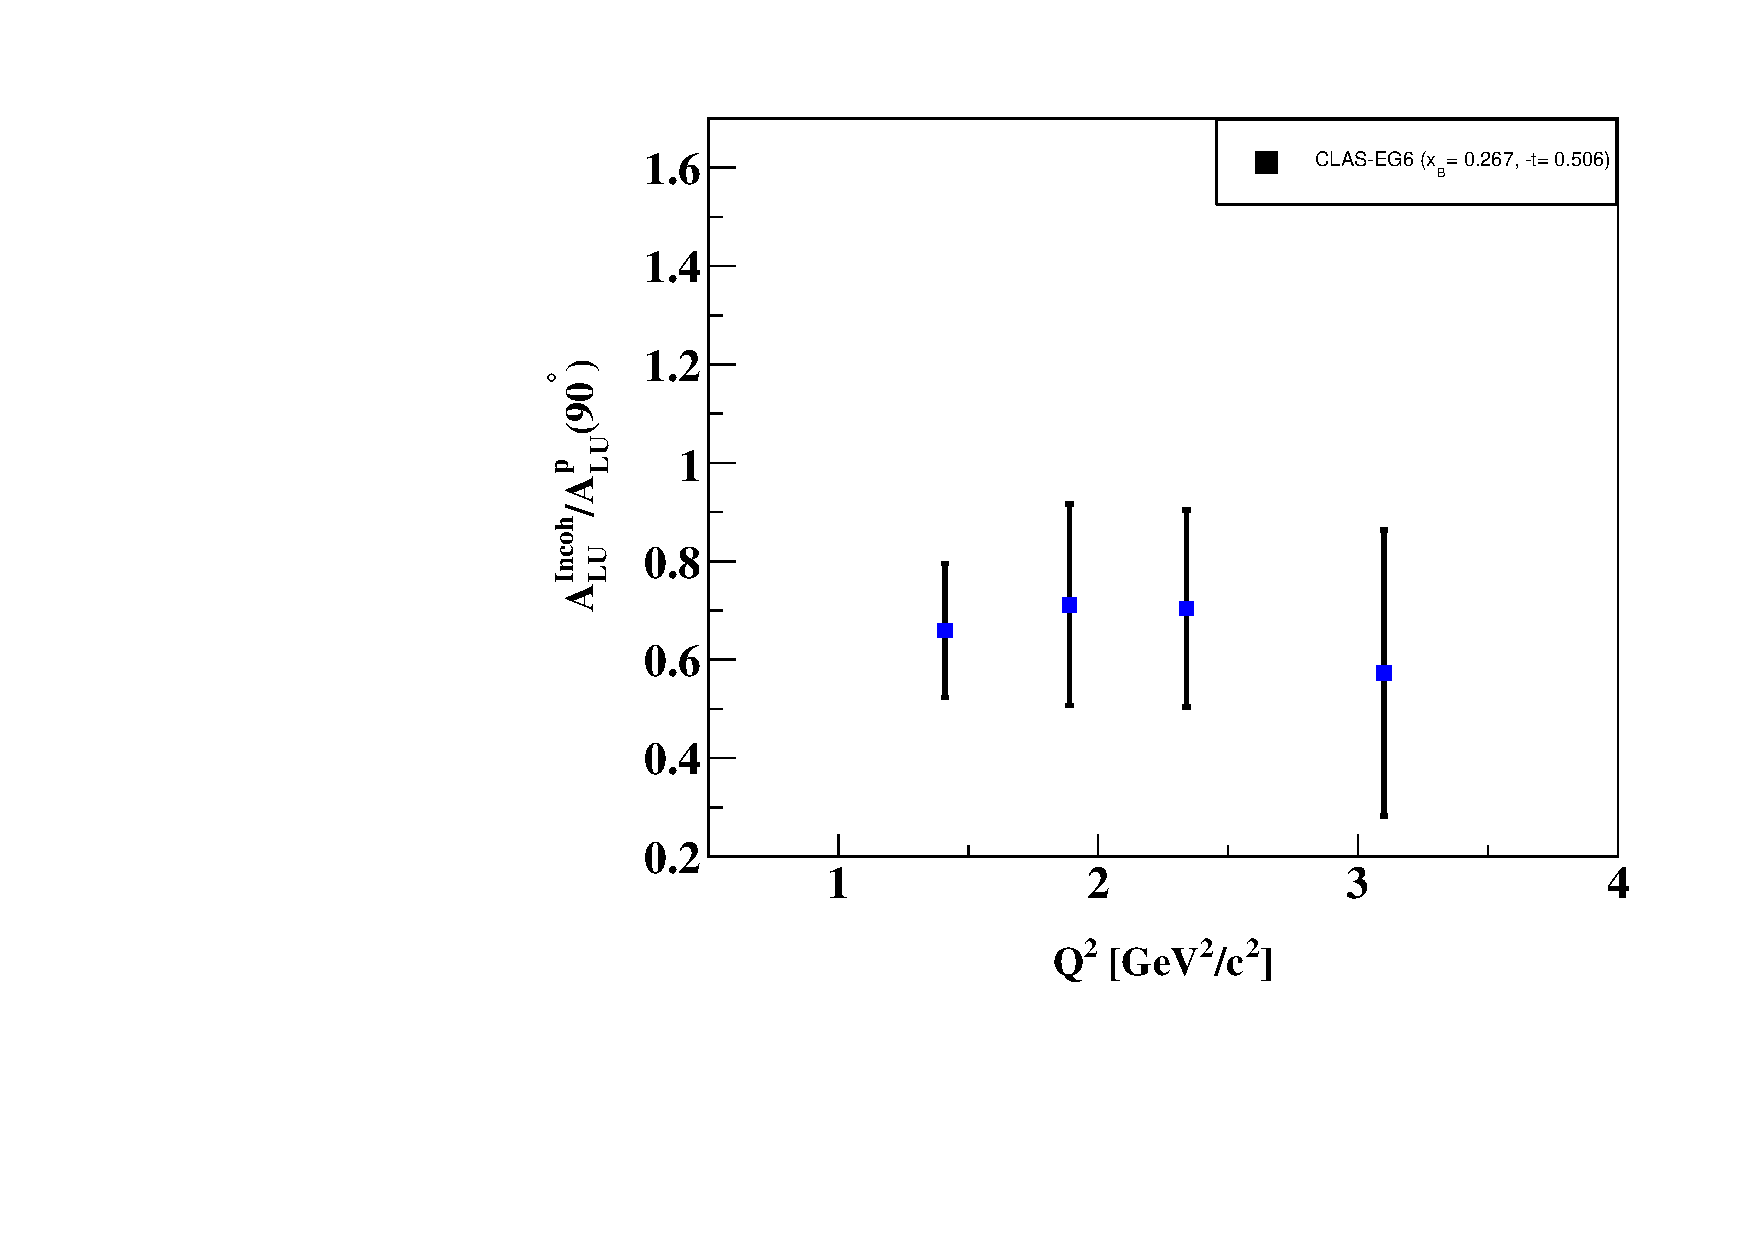
\includegraphics[scale=0.46]{fig_Dec2016/ALU_ratioInc_Q2_shortscenrario.pdf}\\
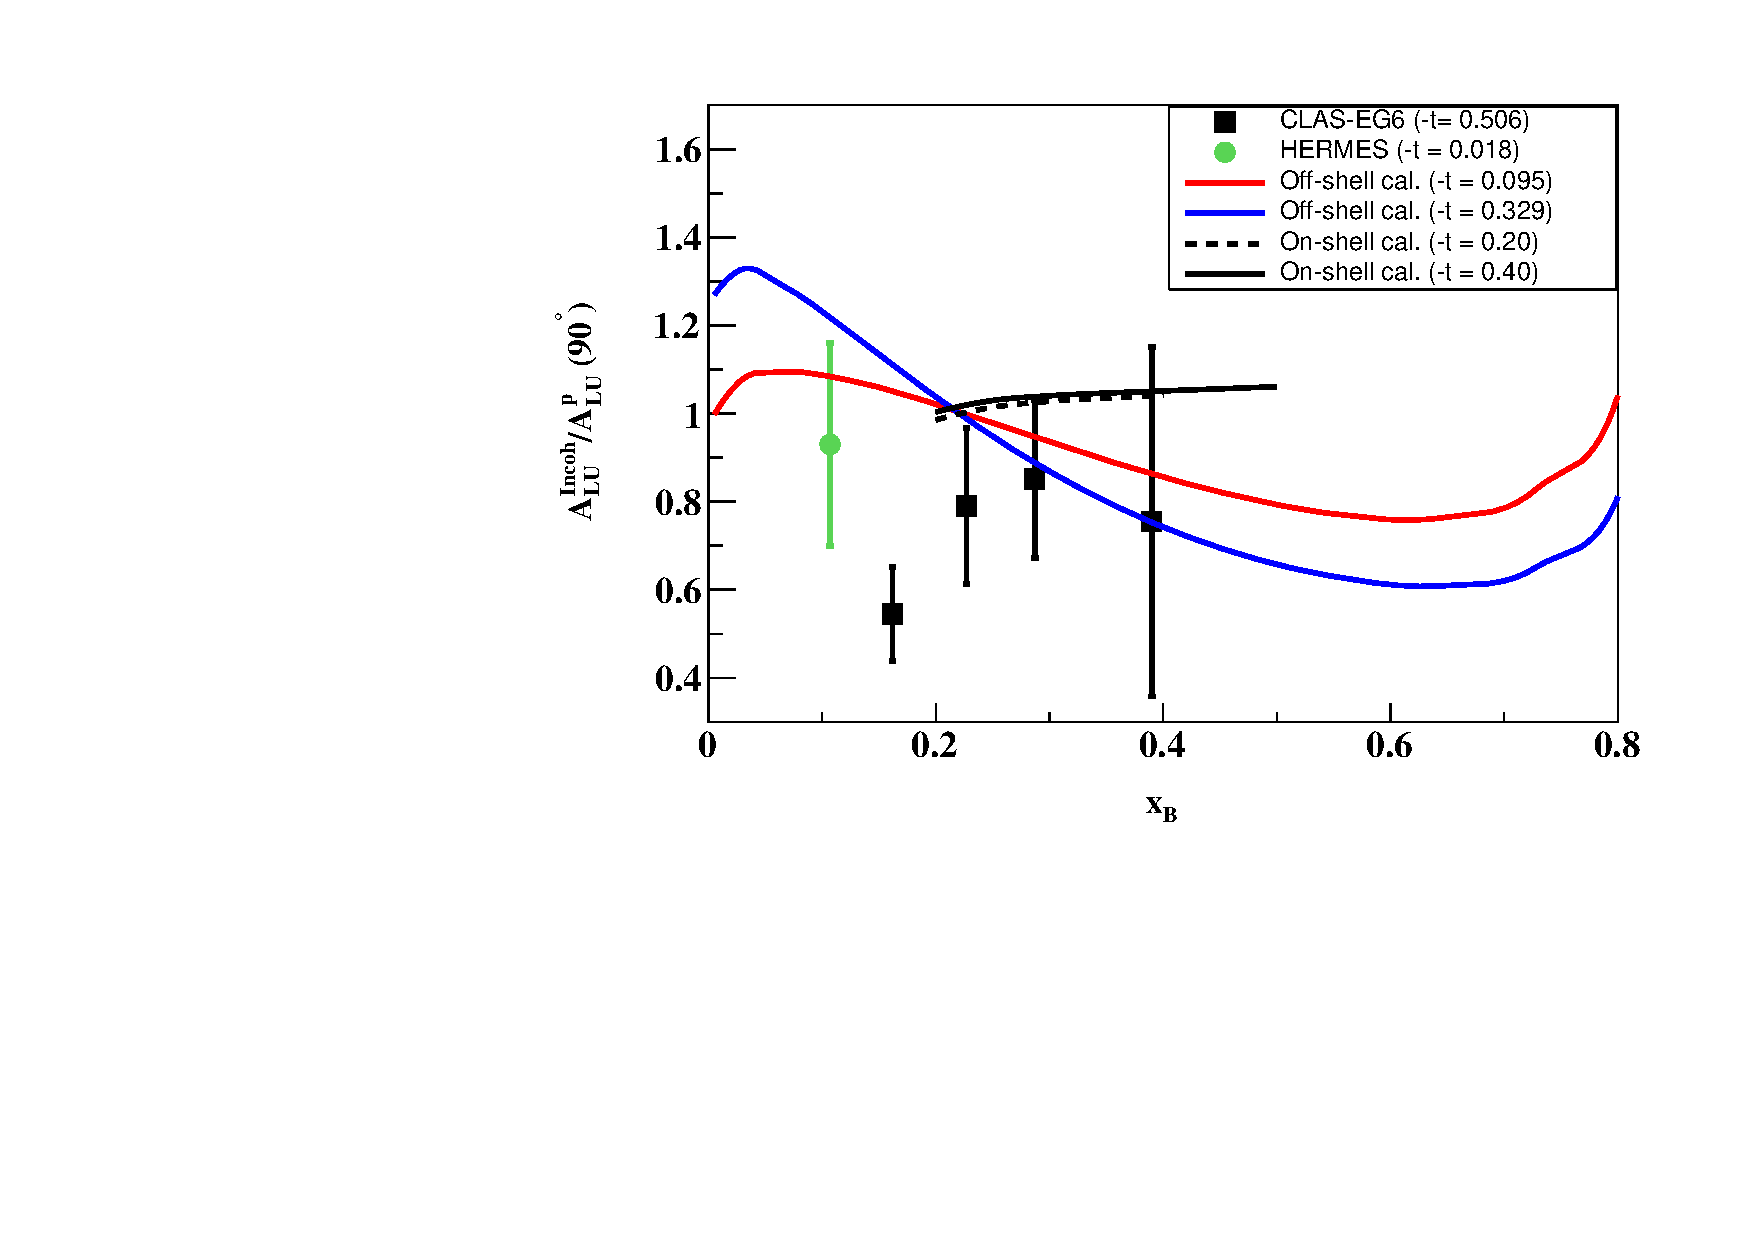
\includegraphics[scale=0.46]{fig_Dec2016/ALU_ratioInc_x_shortscenrario.pdf}\\
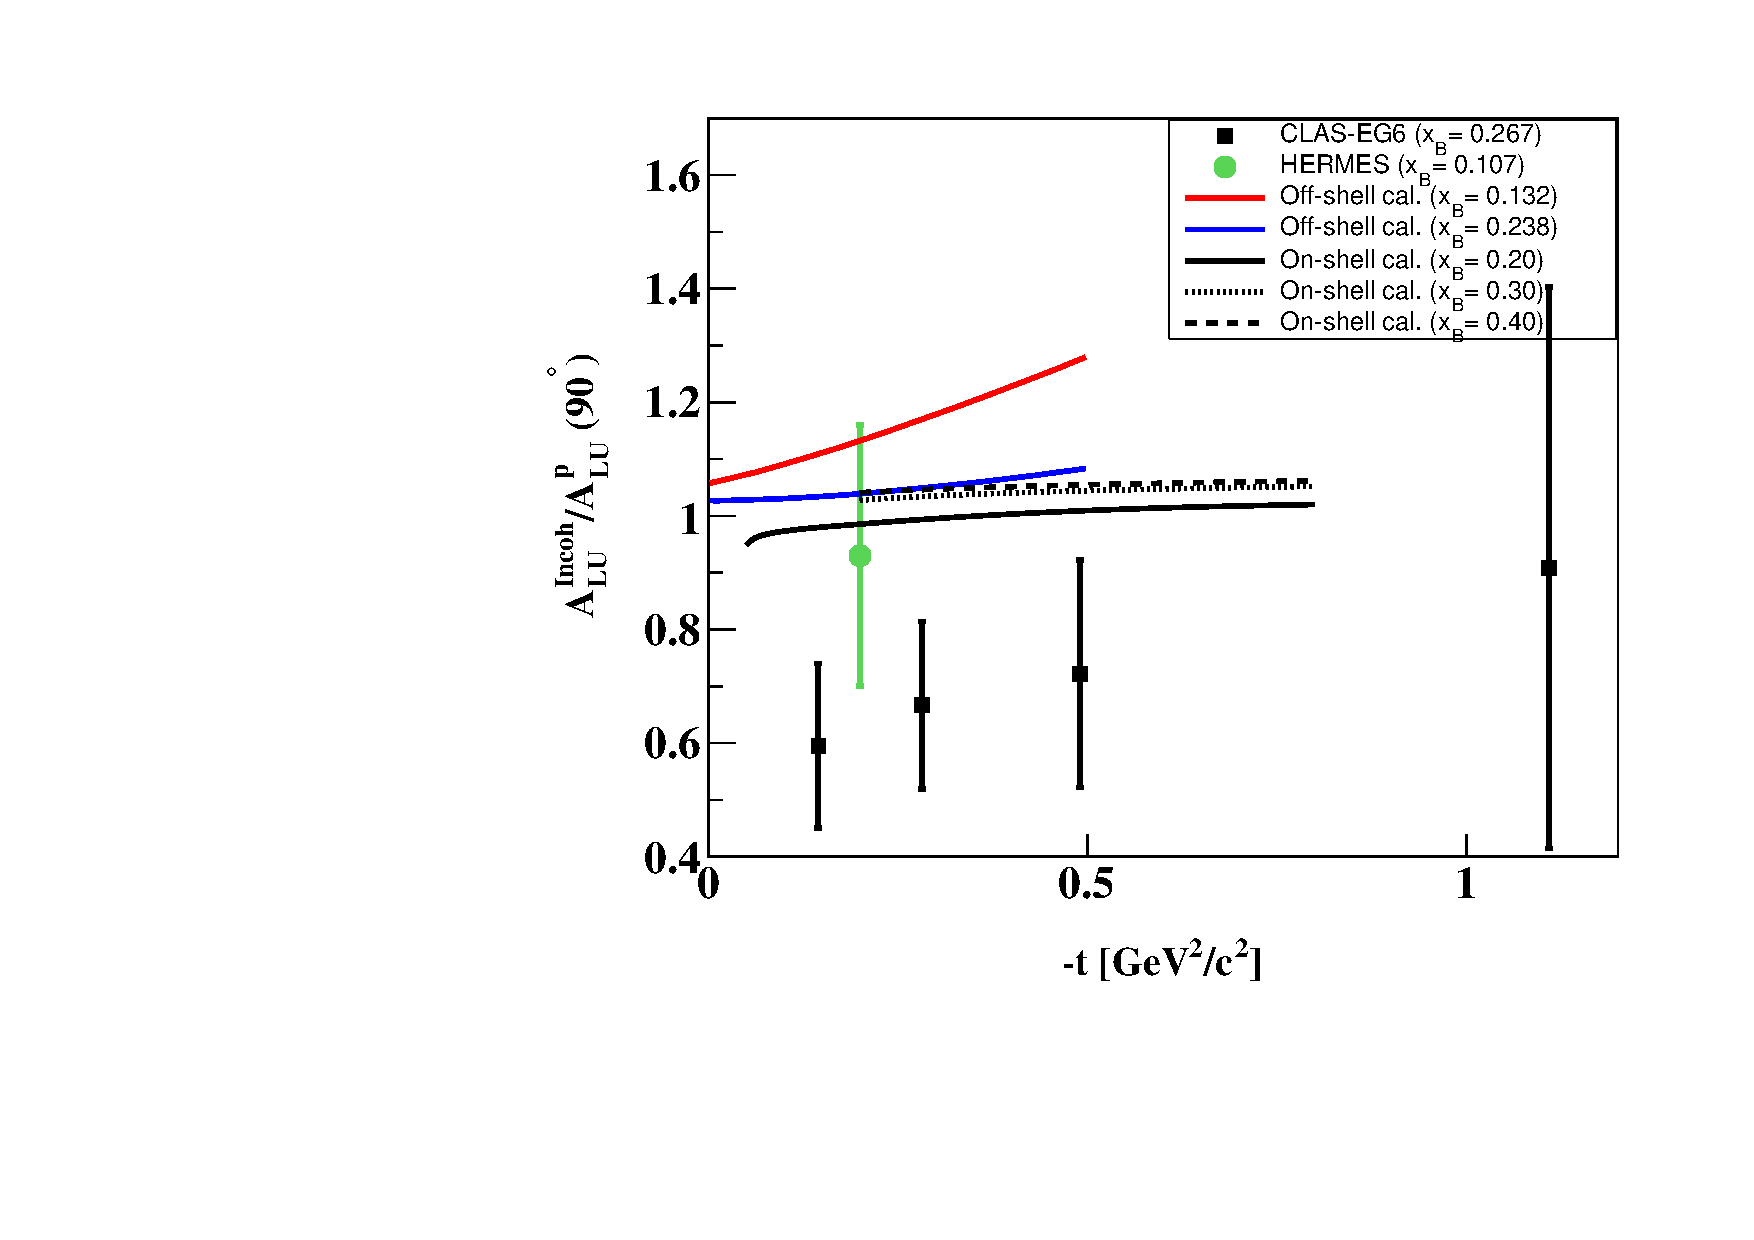
\includegraphics[scale=0.46]{fig_Dec2016/ALU_ratioInc_t_shortscenrario.pdf}
\caption{ The $A_{LU}$ ratio between the bound and the free proton at 
   $\phi$~=~90$^{\circ}$, as a function of $Q^2$ (on the top), $x_B$ (on the 
   middle), and $t$ (on the bottom). The black squares are our results, the 
   green circles are the HERMES inclusive measurement \cite{HERMES_BSA} 
   results.  The blue and red curves are from an on-shell calculations from S.  
Liuti and K. Taneja \cite{simonetta_2}. The solid and dashed black curves are 
from the off-shell calculations \cite{EMC_vadim_2}.} 
\label{fig:incoh_EMC_ratio_ALU_proton}
\end{figure}

Overall the $A_{LU}$ ratios, one can see that the bound protons 
have 20-40$\%$ smaller beam spin asymmetries than the free protons. These measurements 
disagree with the enhancement predicted by the simple impulse approximation of 
V.~Guzey \cite{EMC_vadim_2}, as can be seen in chapter 1, figure 
\ref{fig:EMC_vadim}. The calculations of S. Liuti and K. Taneja \cite{simonetta_2}
also overshoot the data indicating a trend. In particular, the 
anti-shadowing region seems to be absent in terms of the $A_{LU}$ ratio, while
it was predicted by the calculation. Before to draw any strong conclusions on the 
structure of bound protons, it remains to be understood what parasitic
effects can create such a decrease. In particular, final state interactions need
to be evaluated, as they could dilute the signal.  Within the given 
uncertainties, our measured ratios are compatible with the previous measured 
single point from HERMES.


 More attention is needed in constructing the coherent $A_{LU}$ ratio between 
 $^4$He and the free proton. One can see from figure 
 \ref{fig:kinematic_coverage} that the coherent experimental ranges of $Q^2$, 
 $x_{B}$ and $-t$ are limited compared to the incoherent channel especially in 
 the $-t$-domain. The latter is due to the fact that the nuclear form factor of 
 the $^4$He has a steeper drop in $-t$ than the nucleonic one. Our coherent 
 DVCS data set was binned in 3 bins in $Q^{2}$ to show
 $Q^{2}$-dependence of the coherent $A_{LU}$ ratio.  Similar procedures were 
 performed to shows the $x_B$-dependence. For the dependence on $-t$, the data 
 are integrated to one bin to optimize a more precise ratio. The results are 
 presented in figure \ref{fig:coh_EMC_ratio_ALU} along with the available 
 theoretical predictions for this ratio. Our measurements shows a nuclear 
 beam-spin asymmetry enhancement compared to the free proton. 
 The measured ratios are not matching the measurement of 
 HERMES collaboration \cite{HERMES_BSA}, pausing the question of weather they
 actually measured coherent DVCS. It is also in conflict with the calculations 
 of Liuti and K.~Taneja \cite{simonetta_2}, which is missing the large observed 
 increase. On the other hand, our measurements seems to agree with the 
 enhancement predicted by V.~Guzey \cite{EMC_vadim_4}.  Moreover, A.  Kirchner 
 and D. Mueller (KM model) \cite{Kir}, using their formalism of GPDs 
 factorization, have predicted a beam-spin asymmetry ratio of 1.4 (0.35/0.25) 
 for all different spin-zero nuclei at $x_{B}$= 0.3, $E_{b}$= 6GeV, -$t$= 0.25 
 GeV$^2$, and $Q^2$= 2.5 GeV$^2$.  



\begin{figure}[tp]
\centering
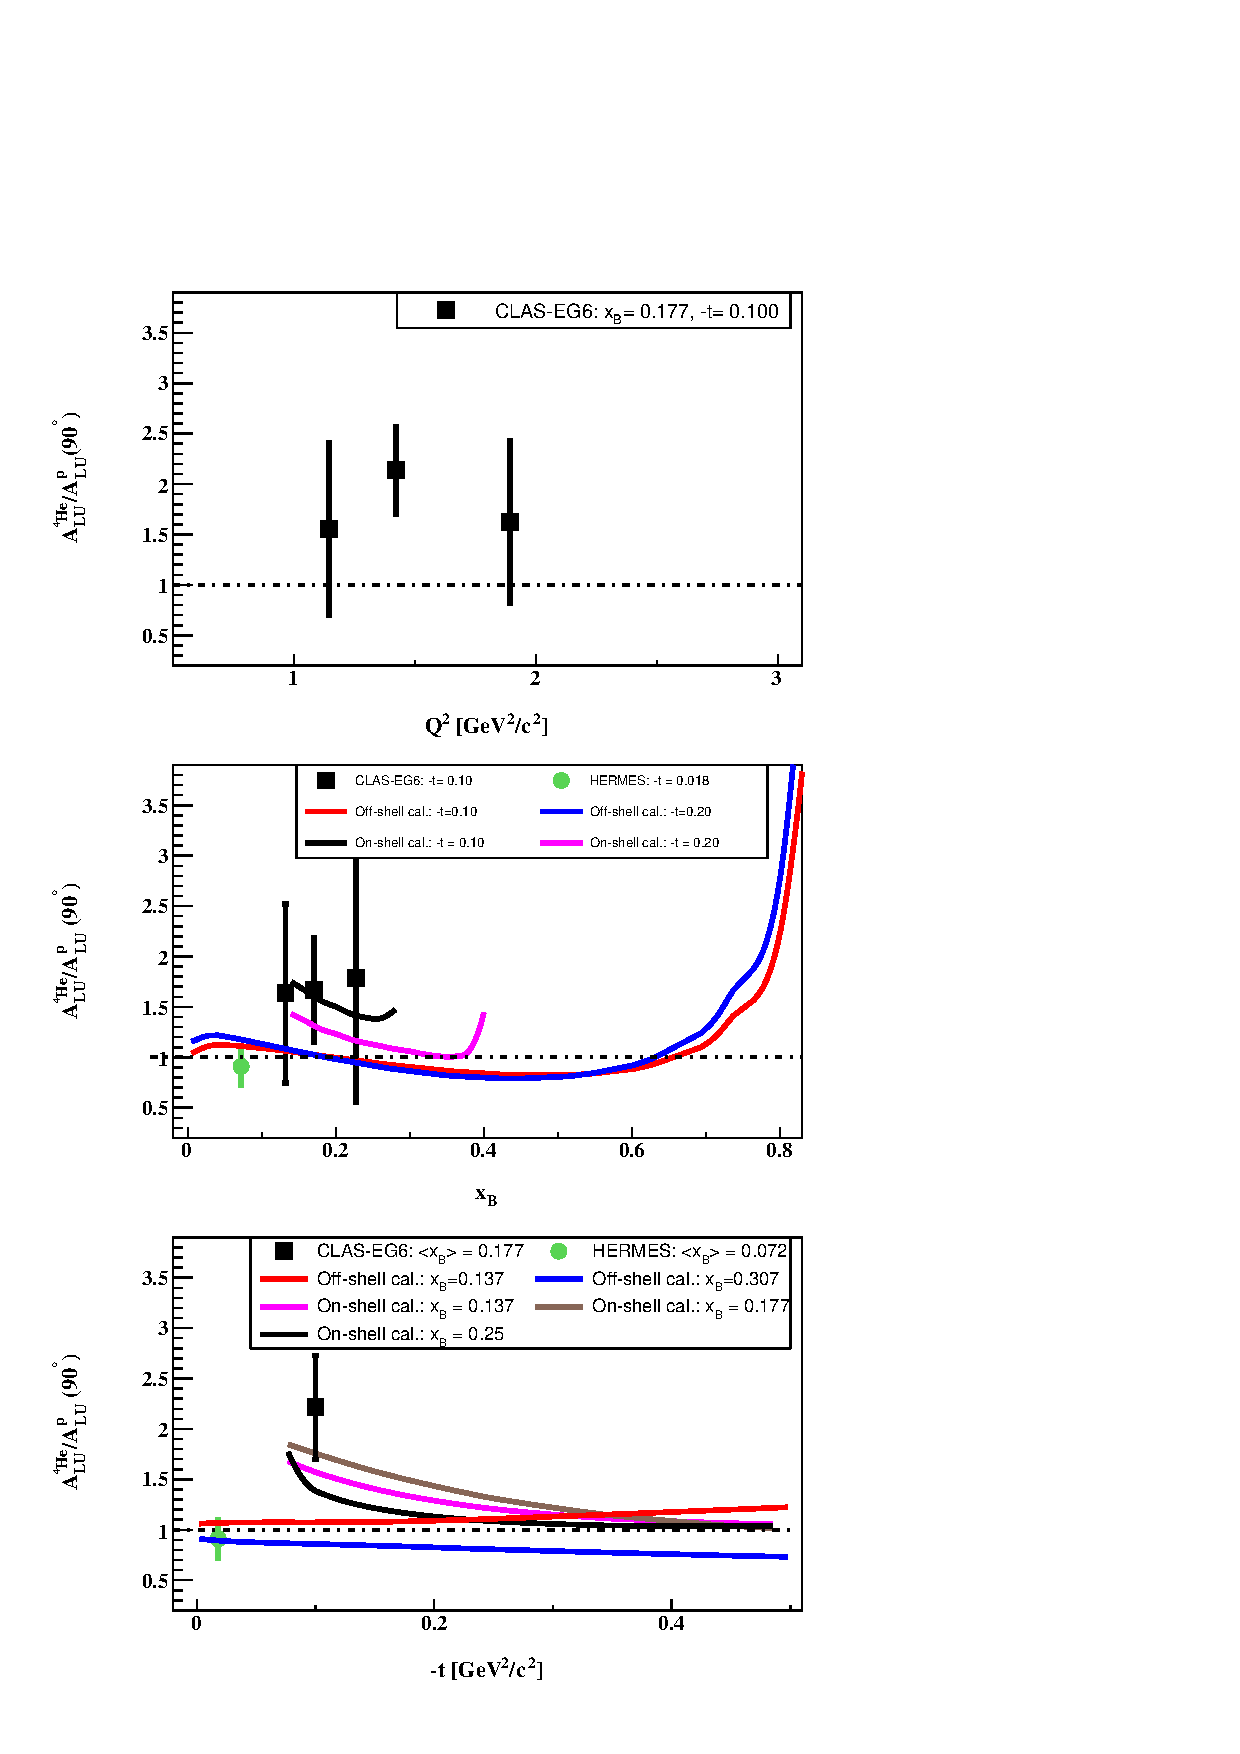
\includegraphics[scale=0.9]{fig_Dec2016/Coherent_ALU_ratio.pdf}\\
\caption{The $A_{LU}$ ratio between $^4$He and free proton at 
   $\phi$~=~90$^{\circ}$, as a function of $Q^2$ (on the top), $x_B$ (on the 
   middle), and $-t$ (on the bottom). The black squares represent the results 
   of this work and the green circles are the HERMES measurements 
   \cite{HERMES_BSA}. These measurements are compared to theoretical 
   predictions from S. Liuti and K. Taneja \cite{simonetta_2}, the red and the 
   blue curves, and the model predictions from V. Guzey et al. based on the 
off-shell calculations \cite{EMC_vadim_4}, in black, purple and brown curves.}
\label{fig:coh_EMC_ratio_ALU}
\end{figure}

  
